\title{Assessment of the pinned specimen digitization progress of the University of Alaska Museum Insect Collection}



\author{by
 Ashley L.\ Smith\footnoteremember{UAM}{University of Alaska Museum, University of Alaska Fairbanks, Fairbanks, Alaska, USA}, 
 Derek S.\ Sikes\footnoterecall{UAM},
 Taylor L.\ Kane\footnoterecall{UAM}, 
 Adam Haberski\footnoterecall{UAM}, 
 Jayce B.\ Williamson\footnoterecall{UAM}, 
 Renee K.\ Nowicki\footnoterecall{UAM} and
 Michael J.\ Apperson\footnoterecall{UAM}
 
 \parbox[t][][s]{\columnwidth}{\vspace{3em}} % This box exists just to prevent the authors from breaking over to a new column.
 }

\maketitle

\end{multicols}

\vspace{-1cm}
\begin{center}
 \parbox[t][][s]{14cm}{\section{Abstract}
 During the Spring semester of 2020, a project was launched to assess the current digitization progress of the pinned \acr{UAM} Insect Collection. The goal was to discover how many specimens were undigitized within each order and rank orders by their digitization completedness to allow strategically targeted digitization efforts. Undigitized specimens represent “dark data,” and by assessing the collection, we hoped to help bring these data into the light so they can be used to answer scientific questions. We examined each drawer of the pinned Insect collection and counted any specimens not bearing a \acr{UAM} barcode label. Upon completion of the initial count, \acr{UAM} staff digitized some of the previously undigitized specimens. The pinned collection is now 90\% digitized. All but four orders are now 100\% digitized. The four orders that are not yet 100\% digitized are Coleoptera (99\%), Hymenoptera (90\%), Diptera (83\%), and Hemiptera (74\%).}
\end{center}

\vspace{4mm}

\begin{multicols}{2}

\section{Introduction} 

As anthropogenic climate change enlarges our planet’s sixth mass extinction crisis \citep{Ceballosetal2015}, there is an increasing urgency to museum science \citep{RavenMiller2020}. Efforts have accelerated to digitize biodiversity data held by the world’s Natural History Collections with a goal of creating open access data according to the \acr{FAIR} Data Principles: findability, accessibility, interoperability, and reusability \citep{NelsonShari2019, Heberlingetal2021}. Many museums have a significant number of specimens whose data are not yet being shared online with the scientific community. Such unshared, undigitized data are often called “dark data” \citep{Heidorn2008, Sikesetal2016}. Dark data are more difficult to access and are consequently often ignored by biodiversity informaticians using so-called ‘Big Data’ to answer questions of conservation concern. For example, \citet{Kerretal2015} analyzed open access, online bumble bee data covering 110 years of collection effort in North America and Europe and detected trends showing range losses and elevational shifts. Specimens with dark data that were relevant to this study were not included because their data were not shared according to \acr{FAIR} data principles.

The University of Alaska Museum Insect Collection (\acr{UAM}) is now over two decades old. \acr{UAM} staff have been able to keep track of and summarize annual growth of the collection’s digitized specimens but had lost track of its undigitized holdings. It is relatively easy to count museum specimen records in a database \citep{Sikes2015, Whitmoreetal2020}, but specimens that are not yet digitized must be counted manually and doing so only provides a snapshot of the undigitized holdings. As work progresses and new specimens are added to the collection and old undigitized specimens are processed, the count of undigitized specimens becomes inaccurate.

In the spring of 2020, we assessed the digitization progress in the \acr{UAM} pinned collection. The purpose of the project was to find out how many specimens were undigitized per insect order.

\section{Methods}

We started at the first drawer of the pinned insect collection and visually counted any specimens not bearing a \acr{UAM} barcode label using a hand-held tally counter. All digitized pinned specimens have a Data Matrix barcode label, which sticks out from under the data label and is visible from above (Figure \ref{barcoded_specimens}). We proceeded through all the drawers in this manner, grouping counts within each order. We did not count parasites or phoretic specimens such as mites or nematomorphs (e.g., \guid{UAM:Ento:354713}) on pinned insect specimens. A pin with multiple specimens of the same taxon on it (e.g., inside a gelatin capsule) was counted as a single undigitized specimen because once digitized it would be a single database record. Our total count is therefore a minimum, not actual, number of pinned specimens \citep{Sikes2015}. 

After we finished a first pass at counting, \acr{UAM} staff used those results to strategically target undigitized specimens for immediate digitization. We therefore present two undigitized counts: the first pass, and the later, most recent counts to show the effectiveness of this strategic approach. We used the most recent counts to calculate the percent digitized for each order and for the entire pinned collection. 

\end{multicols}
\begin{figure}[H]
\begin{center}
\vspace{2mm}
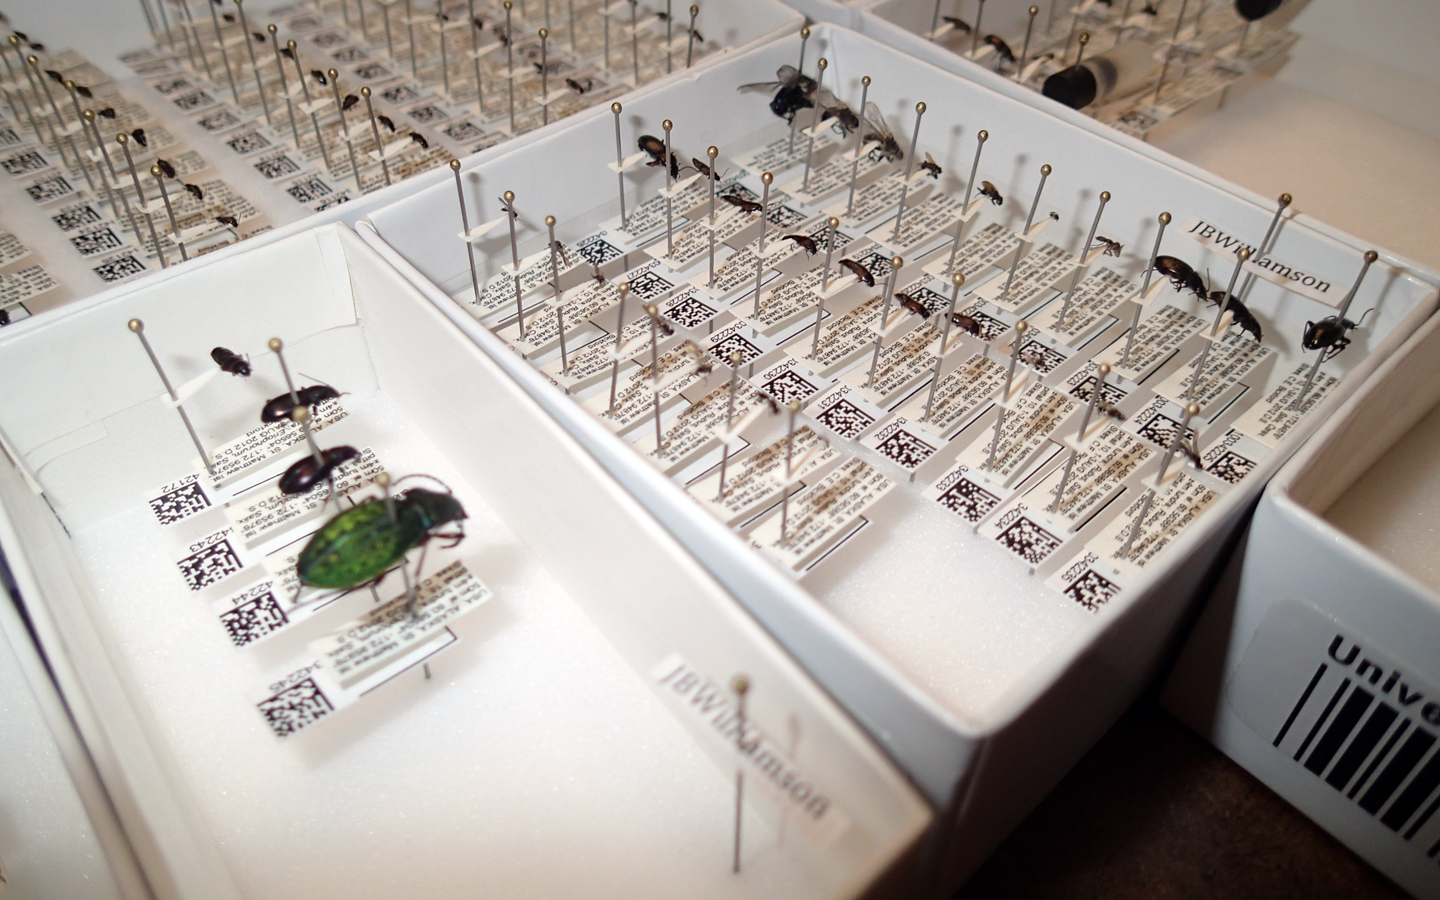
\includegraphics[width=14cm]{img/barcoded_specimens.jpg}
\caption{Example of pinned specimens with \acr{UAM} barcodes visible.}
\label{barcoded_specimens}
\end{center}
\end{figure} 
\begin{multicols}{2} 

\end{multicols}
\begin{center}
\begin{minipage}{\textwidth}
 \setcounter{mpfootnote}{\value{footnote}}
 \renewcommand{\thempfootnote}{\arabic{mpfootnote}}
 \renewcommand\footnoterule{{\hrule height 0pt}}
 \setlength{\footnotemargin}{3.5cm}
\begin{longtable}{lrrrc}

\caption{List of pinned specimens in the UAM Insect Collection by order with initial (1) counts of undigitized specimens from Spring 2020, later current counts (2), current (8 Feb 2021) digital record totals, and percent digitization of each order.\label{digitazationtable}}\\

\hline
\\[-1.0em]
\hline
\\[-1.0em]
\bf{Order} & \bf{Undigitized (1)} & \bf{Undigitized (2)} & \bf{Digitized} &  \bf{\% digitized} \\
\hline
\\[-1.0em]
\endfirsthead

\hline
\bf{Order} & \bf{Undigitized (1)} & \bf{Undigitized (2)} & \bf{Digitized} &  \bf{\% digitized} \\
\hline
\endhead

\multicolumn{5}{c}{\textit{Continued on next page\ldots{}}}\\
\hline
\endfoot

\hline
\\[-1.0em]
\hline
\endlastfoot

Archaeognatha & 0 & 0 & 2 & 100 \\
Blattodea & 3 & 0 & 30 & 100 \\
Coleoptera & 747 & 614 & 75,098 & 99.2 \\
Dermaptera & 0 & 0 & 5 & 100 \\
Diptera & 14,720 & 14,689 & 72,054 & 83.1 \\
Ephemeroptera & 2 & 0 & 36 & 100 \\
Hemiptera & 3,693 & 3,693 & 10,632 & 74.2 \\
Hymenoptera & 7,642 & 7,480 & 69,508 & 90.3 \\
Isoptera & 0 & 0 & 1 & 100 \\
Lepidoptera & 16 & 0 & 14,882 & 100 \\
Mantodea & 0 & 0 & 1 & 100 \\
Mecoptera & 0 & 0 & 2 & 100 \\
Neuroptera & 45 & 0 & 246 & 100 \\
Odonata & 9 & 0 & 116 & 100 \\
Orthoptera & 1,334 & 0 & 2,709 & 100 \\
Plecoptera & 28 & 0 & 110 & 100 \\
Psocodea & 0 & 0 & 47 & 100 \\
Thysanoptera & 0 & 0 & 80 & 100 \\
Trichoptera & 371 & 0 & 854 & 100 \\
Zygentoma & 1 & 0 & 3 & 100 \\
\bf{Totals} & \bf{28,611} & \bf{26,476} & \bf{246,416} & \bf{97.4}\footnote{Averaged.} \\

\end{longtable}
 \setcounter{footnote}{\value{mpfootnote}}
\end{minipage}
\end{center}
\begin{multicols}{2}


\section{Results}

The results in Table \ref{digitazationtable} show that the \acr{UAM} Insect pinned collection holds a minimum total of 272,892 specimens of which a little over 26,000 are not digitized (90.3\% digitized). All small orders, those with fewer than 3,000 specimens, are 100\% digitized. Of the larger orders, Lepidoptera is the most thoroughly digitized (100\%) and Hemiptera the least (74.22\%). 

\section{Discussion}

The most thoroughly digitized large order, Lepidoptera, at 100\% was recently the focus of a large \acr{NSF}-funded “Advancing Digitization of Biological Collections” grant titled LepNet \citep{Seltmannetal2017}, which was intended to complete digitization on all the \acr{UAM} pinned Lepidoptera specimens. Coleoptera, the second most thoroughly digitized order at 99\%, is the taxonomic focus of the curator (second author), and therefore has received more attention than others. However, Coleoptera (75,712 specimens) is only the third largest order in the collection behind Diptera (86,743 specimens) and Hymenoptera (76,988 specimens). The third most thoroughly digitized order, Hymenoptera, at 90\% digitized, grew over the last 6 years from two separate unfunded donations. The first was a large collection of thousands of undigitized parasitoid wasps from the Dominique Collet collection; the second donation was of the Master’s thesis voucher specimens from University of Alaska Fairbanks graduate student Alexandria Wenninger. Together, these donations account for most of the undigitized Hymenoptera specimens. The fourth most thoroughly digitized order, Diptera, at ~83\% digitized, has the largest total number of undigitized specimens (14,689), the bulk of which are from the \acr{USDA} Palmer Agricultural Experiment Station and the Kathryn Sommerman biting fly collections of the mid 20\textsuperscript{th} century. The least thoroughly digitized order, Hemiptera, at 74\% digitized has many drawers of undigitized and unidentified Miridae and Cicadellidae (including many nymphs that are probably unidentifiable) from the \acr{USDA} Palmer Agricultural Experiment Station collection. It is questionable whether these long series of old, unidentified and likely unidentifiable specimens are worth digitizing (or keeping for that matter). Their \acr{DNA} might be of value, and probably the only way to identify most of them, but trying to obtain identifications in this manner would be very costly and a large percentage of specimens might fail to sequence due to degraded \acr{DNA} (raising the cost per successful identification considerably).

The high rate of digitization in the \acr{UAM} Insect Collection is due primarily to the use of the pro-active \acr{DBYL} digitization protocol (Database Before You Label) as described in \citet{Sikesetal2017}. This approach is typically an order of magnitude more efficient than retro-active digitization of already labeled and taxonomically sorted specimens. It ensures that specimens are ‘born digital’ with data captured at the collection event level, and have barcodes and database records before their labels are printed and before they are taxonomically sorted and identified. All the ~26,000 undigitized pinned specimens were prepared using the far less efficient method of typing data into a computer to generate labels (for those prepared in modern times), placing the labels on specimens, sorting taxonomically, and if any digitization happens at all, it is done by reading the data on the labels and typing those data back into a computer one specimen at a time. Assuming that growth of museum collections continues indefinitely into the future, then most specimens have yet to be collected. The last 200+ years of specimen collections will eventually become less than 10\% of the material held in museums. If entomologists wish to maximize the value of limited research funding, they should adopt the \acr{DBYL} protocol, or something similar, to ensure their specimens are ‘born digital’ and do not become a ten-fold cost burden on future generations.

Prior to this project we did not know the size of the pinned insect collection nor what percent was undigitized. Having completed this assessment, the \acr{UAM} Insect Collection is now able to strategically target future digitization efforts to bring these specimens’ “dark data” into the light. We hope to conduct a similar assessment of the alcohol collection in the near future.

\section{Acknowledgments}

This work was completed in fulfillment of the University of Alaska Fairbanks Museum Research Apprenticeship (MRAP 288) course taken by the first author. We thank Kyle Campbell for encouraging the first author to take an MRAP course.
 
\section{Author Contributions}
 
The first author laid eyes on every pinned specimen while counting those that were undigitized, and drafted a report. The second author designed the project and helped with writing and analysis. The remaining authors worked on strategically digitizing specimens after the first pass had been completed and helped review the manuscript.

\bibliography{digitzation}

